%%%%%%%%%%%%%%%%%%%%%%%%%%%%%%%%%%%%%%%%%
% Homework Assignements  
% LaTeX Template
%
% Author:
% Ali Tafakkor
%
%
%%%%%%%%%%%%%%%%%%%%%%%%%%%%%%%%%%%%%%%%%
%
%----------------------------------------------------------------------------------------
%	PACKAGES AND OTHER DOCUMENT CONFIGURATIONS
%----------------------------------------------------------------------------------------

\documentclass[12pt]{article}
\usepackage[margin=25mm]{geometry}
\usepackage[pagebackref=true]{hyperref}
\hypersetup{
    colorlinks,
    citecolor=blue,
    filecolor=blue,
    linkcolor=blue,
    urlcolor=blue
}
\usepackage{tikz}
\usepackage{array}
\usepackage{subcaption}
\usepackage{mathrsfs,amsmath,extarrows}
\usepackage{graphicx}
\usepackage{mathtools}
\usepackage{float}
\usepackage{listings}
\usepackage{hyperref}
\usepackage{xepersian}
\graphicspath{ {images/} }
\settextfont[Scale=0.9]{XB Niloofar}
%\setdigitfont{XB Niloofar}

\begin{document}
\newcommand{\HRule}{\rule{\linewidth}{0.5mm}} % Defines a new command for the horizontal lines, change thickness here
\newcommand\independent{\protect\mathpalette{\protect\independenT}{\perp}}
\def\independenT#1#2{\mathrel{\rlap{$#1#2$}\mkern2mu{#1#2}}}
%----------------------------------------------------------------------------------------
%	HEADING SECTIONS
%----------------------------------------------------------------------------------------

\begin{minipage}[b]{0.65\linewidth}
\begin{center}
\textsc{\LARGE دانشگاه صنعتی خواجه نصیرالدین طوسی}\\[0.3cm]
\textsc{\Large دانشکده مهندسی کامپیوتر}\\[0.5cm]
\textsc{\large طراحی الگوریتم ها - دکتر احمدی}\\[0.5cm]
\textsc{\large نیم‌سال دوم 99-00}\\[0.5cm]
\end{center}
\end{minipage}
\hfill
\begin{minipage}[b]{0.35\linewidth}
\includegraphics[height=8\baselineskip]{kntu_logo.png}
\end{minipage}
%----------------------------------------------------------------------------------------


%----------------------------------------------------------------------------------------
%	TITLE SECTION
%----------------------------------------------------------------------------------------
\begin{center}
\HRule \\[0.4cm]
{ \Large \bfseries پروژه دوم}\\[0.4cm] % Home work series
{ \Large \bfseries  محمّد نامورپور ۹۹۲۰۳۵۴}\\[0.2cm] % Deadline
\HRule \\[0.4cm]
\end{center}

%----------------------------------------------------------------------------------------
%	PROBLEMS
%----------------------------------------------------------------------------------------
\section*{پاراگراف ها}

برای حل این سوال از روش برنامه نویسی پویا
\LTRfootnote{Dynamic Programming}
استفاده کرده ام. 

ابتدا هزینه ی تمام خطوط ممکن را در یک ماتریس به نام
\lr{lineCost}
ذخیره می کنیم.برای این کار از فرمول 
\ref{eq1}
استفاده می کنیم.
\begin{equation}
lineCost(i,j)=(M-(i-j)-\sum_{k=i}^j L_k)^3
\label{eq1}
\end{equation}
 مقدار
$lineCost[i][j]$
نشان می دهد که اگر کلمات $i$ام تا $j$ام در یک خط قرار بگیرند، هزینه چقدر خواهد بود. اگر کلمات $i$ام تا $j$ام نتوانند در یک خط قرار بگیرند (یعنی تعداد کاراکترهایشان از ماکزیمم بیشتر باشد) مقدار
$lineCost[i][j]$
برابر با بی نهایت در نظر گرفته می شود،
\footnote{در کد برای راحتی مقدار بی نهایت را برابر 999999999 در نظر گرفتم}
تا جزئی از راه حل نباشد.

وقتی ماتریس 
\lr{lineCost}
را تکمیل کردیم، هزینه کل را از فرمول بازگشتی زیر باید تعیین کنیم.
\[
    totalCost(j)= 
\begin{cases}
    0,& j = 0\\
    min(lineCost[i-1]+l_c[i,j]),              & j>0
\end{cases}
\]

همانطور که می بینید در فرمول بازگشتی بالا، مثلا پاسخ زیرمسئله 
$totalCost(2)$
توسط 
$totalCost(3)$
و
$totalCost(4)$
استفاده می شود. برنامه نویسی پویا برای ذخیره سازی پاسخ های زیرمسئله ها به کار گرفته شده است.

برای چاپ کردن خروجی، مشخص میکنیم که کدام کلمات در کدام خطوط قرار میگیرند. برای این منظور از لیست 
$solution$
استفاده کرده ایم که نشان می دهد هر مقدار در لیست 
$totalCost$
از کجا آمده است. 

\subsection*{پیچیدگی زمانی}
در قسمتی که میخواهیم ماتریس 
$lineCost$
را تکمیل کنیم، دو حلقه تو در تو داریم که هر کدام از $0$ تا $n+1$ را می پیمایند.

پس در صورتی که $n$ کلمه به الگوریتم داده شود، پیچیدگی زمانی الگوریتم نیز 
$O(n^2)$
خواهد بود.

\subsection*{تصویری از اجرای برنامه}
شکل
\ref{fig1}
تصویری از اجرای برنامه برای جمله آزمایشی
\lr{With great power comes great responsibility}
است.

\begin{figure}[H]
	\centering
	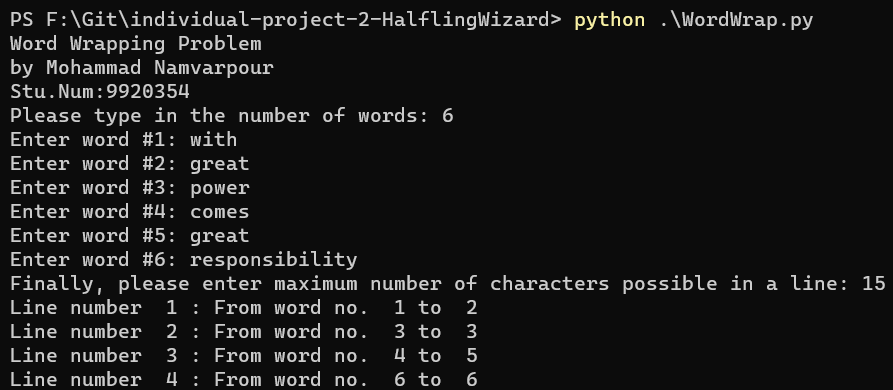
\includegraphics[width=.4\linewidth]{run.png}
	\caption{اجرای برنامه برای جمله آزمایشی
\lr{With great power comes great responsibility}}
	\label{fig1}
\end{figure}
\end{document}